\chapter{Preliminaries}
The work presented in this document borrows many conepts, techniques, and results from linear algebra and linear systems theory. Because these topics are later presented without discussion, we present an overview of them here. This overview is not intended to provide a comprehensive discussion of these topics, rather it serves to introduce the reader to the general topics as they are used in this document.

\section{Vector and Matrix Notation}
We define $\mathbb{R}$ be the set of reals, $\mathbb{R}^n$ the set of $n$-dimensional real vectors, and $\mathbb{R}^{m\times n}$ the set of real matrices. We denote vectors by lower case letters $\{a$, $b$, $c$, $\dots\}$ and matrices by upper case letters $\{A$, $B$, $C$, $\dots\}$. Transpositions of vectors and matrices are denoted by $a^T$ and $A^T$, respectively. The inverse of a square matrix $A$ is denoted $A^{-1}$ and its Moore-Penrose psedudoinverse is denoted by $A^\dagger$.

\section{Linear Systems}
\subsection{Linear Time-Invariant Systems}\label{sec:linear_time_invariant_systems}
A discrete time state space representation of a linear dynamical system can be written as
\begin{subequations}\label{eq:2_lti_state_space}
\begin{equation}x(k+1) = Ax(k) + Bu(k)\end{equation}
\begin{equation}y(k) = Cx(k) + Du(k)\end{equation}
\end{subequations}
where $x(k) \in \mathbb{R}^n$ is a vector of the states of the system, $u(k) \in \mathbb{R}^m$ is a vector of input signals, $y(k) \in \mathbb{R}^l$ is a vector of output signals, and  $k \in \mathbb{Z}$ is the time index. $A$, $B$, $C$, and $D$ are the system matrices with dimensions $A\in\mathbb{R}^{n\times n}$, $B\in\mathbb{R}^{n\times m}$, $C\in\mathbb{R}^{l\times n}$, $D\in\mathbb{R}^{l\times m}$.
\begin{figure}[htb!]
	\centering
	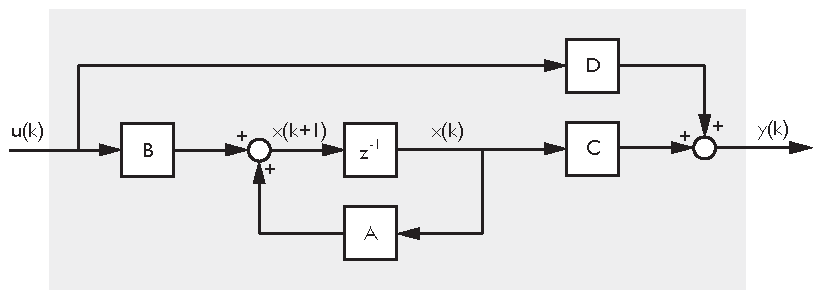
\includegraphics{../fig/lti_block_diagram.pdf}
	\caption{A block diagram of the state space representation of a LTI system.}
\end{figure}

For any state space representation of a system, the state sequence is not unique. That is, there are different state space representations resulting in the same input-output behavior of the system. These differing states can be related by a similarity transform $T$ where $T$ is a real, nonsingular matrix
\begin{equation*}
\tilde{x}(k) = T^{-1}x(k)
\end{equation*}
where the tilde in $\tilde x$ indicates that it is ``similar'' to the original state sequence $x$. The state space representation of the system corresponding to the transformed state $\tilde{x}$ is given by
\begin{subequations}
\begin{equation*}\tilde{x}(k+1) = \tilde{A}\tilde{x}(k) + \tilde{B}u(k)\end{equation*}
\begin{equation*}y(k) = \tilde{C}\tilde{x}(k) + \tilde{D}u(k)\end{equation*}
\end{subequations}
where
\begin{equation*}
\tilde{A} = T^{-1}AT, \qquad
\tilde{B} = T^{-1}B, \qquad
\tilde{C} = CT, \qquad
\tilde{D} = D
\end{equation*}

\subsection{Stability}
The LTI system given by $A$, $B$, $C$, $D$ is said to be \textit{stable} if all the eigenvalues of $A$ lie strictly within the unit circle on the complex plane. The system response of a stable LTI system asymptotically converges to a steady state value.

\subsection{Observability and Controllability}
The LTI system given by $A$, $B$, $C$, $D$ or equivalently the pair $(A,C)$ is said to be \textit{observable} if for any finite time $t_1 > 0$, the initial state $x(0) = x_0$ can be uniquely determined from measurements of the input $u$ and output $y$ over the interval $[0, t_1], t_1>0$.

The LTI system given by $A$, $B$, $C$, $D$ or equivalently the pair $(A,B)$ is said to be \textit{controllable} if for any final state $x_1$ there exists an input sequence $u_k$ defined on the interval $[0, t_1], t_1>0$ that transfers the state from $x(0) = x_0$ to $x_1$ in finite time.

LTI systems $A$, $B$, $C$, $D$ in state space form which are both observable and controllable are said to be \textit{minimal}, meaning that the matrix $A$ has the smallest possible dimension.

\subsection{Combined Deterministic-Stochastic LTI Systems}
Section \ref{sec:linear_time_invariant_systems} considered the case of a purely deterministic LTI system; that is, a system operating in a noise-free environment. In practice, this rarely happens so we now consider the case of the combined deterministic-stochastic LTI system operating in the presence of process and measurement noise. We append Eq. \ref{eq:2_lti_state_space} as follows:
\begin{subequations}\label{eq:2_lti_noise}
\begin{equation}x(k+1) = Ax(k) + Bu(k) + w(k)\end{equation}
\begin{equation}y(k) = Cx(k) + Du(k) + v(k)\end{equation}
\end{subequations}
where $w(k)\in\mathbb{R}^1$ is the process noise and $v(k)\in\mathbb{R}^1$ is the measurement noise. As is commonly done, we assume $w(k)$ and $v(k)$ are zero-mean white-noise sequences. 

If the system is observable, we can design a Kalman filter to estimate the system state \cite{kalman1960new}
\begin{equation*}
\hat{x}(k+1) = A\hat{x}(k) + Bu(k) + K\big(y(k) - C\hat{x}(k) - Du(k)\big)
\end{equation*}
where $K$ is the Kalman filter gain. If we denote 
\begin{equation*}
e(k) = y(k) - C\hat{x}(k) - Du(k)
\end{equation*}
to be the innovation sequence, we can rewrite the combined deterministic-stochastic system in Eq. (\ref{eq:2_lti_noise}) in the following equivalent \textit{innovation form}:
\begin{subequations}\label{eq:2_innovation}
\begin{equation}x(k+1) = Ax(k) + Bu(k) + Ke(k)\end{equation}
\begin{equation}y(k) = Cx(k) + Du(k) + e(k)\end{equation}
\end{subequations}

\section{Linear Algebra Tools}

\subsection{Fundamental Matrix Subspaces}
We require two of the fundamental matrix subspaces: \textit{column space} and \textit{row space}. The column space of a matrix $A \in \mathbb{R}^{m\times n}$ is the set of all linear combinations of the column vectors of $A$, sometimes called the range of $A$. The dimension of the column space is called the rank of $A$. The row space of a matrix $B \in \mathbb{R}^{m\times n}$ is the set of all linear combinations of the row vectors of $B$.


\subsection{Orthogonal Projections}
The \textit{orthogonal projection} of the row space of $A$ onto the row space of $B$ is $A\Pi_B$, defined as
\begin{equation*}
A\Pi_B = AB^T(BB^T)^{-1}B
\end{equation*}
The projection of the row space of $A$ onto the orthogonal compliment of the row space of $B$ is $A\Pi_B^\perp$, defined as
\begin{equation*}
A\Pi_B^\perp = A\big(I-B^T(BB^T)^{-1}B\big)
\end{equation*}
\begin{figure}[htb!]
	\centering
	
\includegraphics{../fig/orthogonal_projection.pdf}
	\caption{Orthogonal projections of $A$ onto $B$ and $A$ onto the orthogonal compliment of $B$.}
\end{figure}

Additionally, we define the following properties of orthogonal projections:
\begin{equation*}
B\Pi_B = BB^T(BB^T)^{-1}B = B
\end{equation*}
\begin{equation*}
B\Pi_B^\perp = B\big(I-B^T(BB^T)^{-1}B\big) = B-B = 0
\end{equation*}

When $B$ is large, computing its inverse and thus orthogonal projections onto its subspace is computationally intensive. A more numerically efficient computation of of an orthogonal projection is achieved by LQ decomposition. From the LQ decomposition
\begin{equation*}
\begin{bmatrix}B\\A\end{bmatrix} = 
\begin{bmatrix}L_{11} & 0\\ L_{21} & L_{22}\end{bmatrix}
\begin{bmatrix}Q_1\\ Q_2\end{bmatrix}
\end{equation*}
we have
\begin{equation*}
A\Pi_B = L_{21}Q_1
\end{equation*}
\begin{equation*}
A\Pi_B^\perp = L_{22}Q_2
\end{equation*}

\subsection{Singular Value Decomposition}
Any matrix $A \in \mathbb{R}^{m\times n}$ can be decomposed by a singular value decomposition (SVD) given by
\begin{equation*}
A = U\Sigma V^T
\end{equation*}
where $U \in \mathbb{R}^{m\times m}$ and $V \in \mathbb{R}^{n\times n}$ are orthogonal matrices and $\Sigma \in \mathbb{R}^{m\times n}$ is diagonal matrix of the singular values $\sigma_i$ of $A$, ordered such that
\begin{equation*}
\sigma_1 \geq \sigma_2 \geq \cdots \geq \sigma_r > 0
\end{equation*}
If we partition the matrices in the SVD as
\begin{equation*}
A = \left[\begin{array}{c|c}
U_1 & U_2
\end{array}\right]
\left[\begin{array}{c|c}
\Sigma_r & 0 \\ \hline 0 & 0
\end{array}\right]
\left[\begin{array}{c}
V_1^T \\ \hline V_2^T
\end{array}\right]
\end{equation*}
a well known property of the SVD is that the vectors $U_1$ corresponding to the $r$ non-zero singular values of $A$ span the range of $A$. That is,
\begin{equation*}
\mbox{range}(U_1) = \mbox{range}(A)
\end{equation*}

\subsection{Hankel Matrices}
A Hankel matrix is a matrix $A \in \mathbb{R}^{m\times n}$ with constant skew-diagonals:
\begin{equation*}
A_{m,n} = \begin{bmatrix}
a_1 & a_2 & \cdots & a_n\\
a_2 & a_3 & \cdots & a_{n+1}\\
\vdots & \vdots & \ddots & \vdots\\
a_m & a_{m+1} & \cdots & a_{m+n-1}
\end{bmatrix}
\end{equation*}
Hankel matrices can be constructed by setting the $(i,j)^{\mbox{th}}$ element of $A$ to
\begin{equation*}
A_{i,j} = A_{i-1, j+1}
\end{equation*}
If each entry in the matrix is also a matrix, the resulting matrix is called a block Hankel matrix:


\subsection{Toeplitz Matrices}
A Toeplitz matrix is a matrix $A\in\mathbb{R}^{m\times n}$ with constant diagonals. 
\begin{equation*}
A_{m,n} = \begin{bmatrix}
a_1 & a_{-1} & \cdots & a_{-n+1}\\
a_2 & a_1 & \ddots & \vdots\\
\vdots & \ddots & \ddots & a_{-1}\\
a_{m-1} & \cdots & a_2 & a_1
\end{bmatrix}
\end{equation*}
Topelitz matrices can be constructed by setting the $(i,j)^{\mbox{th}}$ element of $A$ to
\begin{equation*}
A_{i,j} = A_{i+1, j+1}
\end{equation*}
